% Options for packages loaded elsewhere
\PassOptionsToPackage{unicode}{hyperref}
\PassOptionsToPackage{hyphens}{url}
\PassOptionsToPackage{dvipsnames,svgnames,x11names}{xcolor}
%
\documentclass[
  letterpaper,
  DIV=11,
  numbers=noendperiod]{scrartcl}

\usepackage{amsmath,amssymb}
\usepackage{iftex}
\ifPDFTeX
  \usepackage[T1]{fontenc}
  \usepackage[utf8]{inputenc}
  \usepackage{textcomp} % provide euro and other symbols
\else % if luatex or xetex
  \usepackage{unicode-math}
  \defaultfontfeatures{Scale=MatchLowercase}
  \defaultfontfeatures[\rmfamily]{Ligatures=TeX,Scale=1}
\fi
\usepackage{lmodern}
\ifPDFTeX\else  
    % xetex/luatex font selection
\fi
% Use upquote if available, for straight quotes in verbatim environments
\IfFileExists{upquote.sty}{\usepackage{upquote}}{}
\IfFileExists{microtype.sty}{% use microtype if available
  \usepackage[]{microtype}
  \UseMicrotypeSet[protrusion]{basicmath} % disable protrusion for tt fonts
}{}
\makeatletter
\@ifundefined{KOMAClassName}{% if non-KOMA class
  \IfFileExists{parskip.sty}{%
    \usepackage{parskip}
  }{% else
    \setlength{\parindent}{0pt}
    \setlength{\parskip}{6pt plus 2pt minus 1pt}}
}{% if KOMA class
  \KOMAoptions{parskip=half}}
\makeatother
\usepackage{xcolor}
\setlength{\emergencystretch}{3em} % prevent overfull lines
\setcounter{secnumdepth}{-\maxdimen} % remove section numbering
% Make \paragraph and \subparagraph free-standing
\ifx\paragraph\undefined\else
  \let\oldparagraph\paragraph
  \renewcommand{\paragraph}[1]{\oldparagraph{#1}\mbox{}}
\fi
\ifx\subparagraph\undefined\else
  \let\oldsubparagraph\subparagraph
  \renewcommand{\subparagraph}[1]{\oldsubparagraph{#1}\mbox{}}
\fi

\usepackage{color}
\usepackage{fancyvrb}
\newcommand{\VerbBar}{|}
\newcommand{\VERB}{\Verb[commandchars=\\\{\}]}
\DefineVerbatimEnvironment{Highlighting}{Verbatim}{commandchars=\\\{\}}
% Add ',fontsize=\small' for more characters per line
\usepackage{framed}
\definecolor{shadecolor}{RGB}{241,243,245}
\newenvironment{Shaded}{\begin{snugshade}}{\end{snugshade}}
\newcommand{\AlertTok}[1]{\textcolor[rgb]{0.68,0.00,0.00}{#1}}
\newcommand{\AnnotationTok}[1]{\textcolor[rgb]{0.37,0.37,0.37}{#1}}
\newcommand{\AttributeTok}[1]{\textcolor[rgb]{0.40,0.45,0.13}{#1}}
\newcommand{\BaseNTok}[1]{\textcolor[rgb]{0.68,0.00,0.00}{#1}}
\newcommand{\BuiltInTok}[1]{\textcolor[rgb]{0.00,0.23,0.31}{#1}}
\newcommand{\CharTok}[1]{\textcolor[rgb]{0.13,0.47,0.30}{#1}}
\newcommand{\CommentTok}[1]{\textcolor[rgb]{0.37,0.37,0.37}{#1}}
\newcommand{\CommentVarTok}[1]{\textcolor[rgb]{0.37,0.37,0.37}{\textit{#1}}}
\newcommand{\ConstantTok}[1]{\textcolor[rgb]{0.56,0.35,0.01}{#1}}
\newcommand{\ControlFlowTok}[1]{\textcolor[rgb]{0.00,0.23,0.31}{#1}}
\newcommand{\DataTypeTok}[1]{\textcolor[rgb]{0.68,0.00,0.00}{#1}}
\newcommand{\DecValTok}[1]{\textcolor[rgb]{0.68,0.00,0.00}{#1}}
\newcommand{\DocumentationTok}[1]{\textcolor[rgb]{0.37,0.37,0.37}{\textit{#1}}}
\newcommand{\ErrorTok}[1]{\textcolor[rgb]{0.68,0.00,0.00}{#1}}
\newcommand{\ExtensionTok}[1]{\textcolor[rgb]{0.00,0.23,0.31}{#1}}
\newcommand{\FloatTok}[1]{\textcolor[rgb]{0.68,0.00,0.00}{#1}}
\newcommand{\FunctionTok}[1]{\textcolor[rgb]{0.28,0.35,0.67}{#1}}
\newcommand{\ImportTok}[1]{\textcolor[rgb]{0.00,0.46,0.62}{#1}}
\newcommand{\InformationTok}[1]{\textcolor[rgb]{0.37,0.37,0.37}{#1}}
\newcommand{\KeywordTok}[1]{\textcolor[rgb]{0.00,0.23,0.31}{#1}}
\newcommand{\NormalTok}[1]{\textcolor[rgb]{0.00,0.23,0.31}{#1}}
\newcommand{\OperatorTok}[1]{\textcolor[rgb]{0.37,0.37,0.37}{#1}}
\newcommand{\OtherTok}[1]{\textcolor[rgb]{0.00,0.23,0.31}{#1}}
\newcommand{\PreprocessorTok}[1]{\textcolor[rgb]{0.68,0.00,0.00}{#1}}
\newcommand{\RegionMarkerTok}[1]{\textcolor[rgb]{0.00,0.23,0.31}{#1}}
\newcommand{\SpecialCharTok}[1]{\textcolor[rgb]{0.37,0.37,0.37}{#1}}
\newcommand{\SpecialStringTok}[1]{\textcolor[rgb]{0.13,0.47,0.30}{#1}}
\newcommand{\StringTok}[1]{\textcolor[rgb]{0.13,0.47,0.30}{#1}}
\newcommand{\VariableTok}[1]{\textcolor[rgb]{0.07,0.07,0.07}{#1}}
\newcommand{\VerbatimStringTok}[1]{\textcolor[rgb]{0.13,0.47,0.30}{#1}}
\newcommand{\WarningTok}[1]{\textcolor[rgb]{0.37,0.37,0.37}{\textit{#1}}}

\providecommand{\tightlist}{%
  \setlength{\itemsep}{0pt}\setlength{\parskip}{0pt}}\usepackage{longtable,booktabs,array}
\usepackage{calc} % for calculating minipage widths
% Correct order of tables after \paragraph or \subparagraph
\usepackage{etoolbox}
\makeatletter
\patchcmd\longtable{\par}{\if@noskipsec\mbox{}\fi\par}{}{}
\makeatother
% Allow footnotes in longtable head/foot
\IfFileExists{footnotehyper.sty}{\usepackage{footnotehyper}}{\usepackage{footnote}}
\makesavenoteenv{longtable}
\usepackage{graphicx}
\makeatletter
\def\maxwidth{\ifdim\Gin@nat@width>\linewidth\linewidth\else\Gin@nat@width\fi}
\def\maxheight{\ifdim\Gin@nat@height>\textheight\textheight\else\Gin@nat@height\fi}
\makeatother
% Scale images if necessary, so that they will not overflow the page
% margins by default, and it is still possible to overwrite the defaults
% using explicit options in \includegraphics[width, height, ...]{}
\setkeys{Gin}{width=\maxwidth,height=\maxheight,keepaspectratio}
% Set default figure placement to htbp
\makeatletter
\def\fps@figure{htbp}
\makeatother

\KOMAoption{captions}{tableheading}
\makeatletter
\makeatother
\makeatletter
\makeatother
\makeatletter
\@ifpackageloaded{caption}{}{\usepackage{caption}}
\AtBeginDocument{%
\ifdefined\contentsname
  \renewcommand*\contentsname{Table of contents}
\else
  \newcommand\contentsname{Table of contents}
\fi
\ifdefined\listfigurename
  \renewcommand*\listfigurename{List of Figures}
\else
  \newcommand\listfigurename{List of Figures}
\fi
\ifdefined\listtablename
  \renewcommand*\listtablename{List of Tables}
\else
  \newcommand\listtablename{List of Tables}
\fi
\ifdefined\figurename
  \renewcommand*\figurename{Figure}
\else
  \newcommand\figurename{Figure}
\fi
\ifdefined\tablename
  \renewcommand*\tablename{Table}
\else
  \newcommand\tablename{Table}
\fi
}
\@ifpackageloaded{float}{}{\usepackage{float}}
\floatstyle{ruled}
\@ifundefined{c@chapter}{\newfloat{codelisting}{h}{lop}}{\newfloat{codelisting}{h}{lop}[chapter]}
\floatname{codelisting}{Listing}
\newcommand*\listoflistings{\listof{codelisting}{List of Listings}}
\makeatother
\makeatletter
\@ifpackageloaded{caption}{}{\usepackage{caption}}
\@ifpackageloaded{subcaption}{}{\usepackage{subcaption}}
\makeatother
\makeatletter
\@ifpackageloaded{tcolorbox}{}{\usepackage[skins,breakable]{tcolorbox}}
\makeatother
\makeatletter
\@ifundefined{shadecolor}{\definecolor{shadecolor}{rgb}{.97, .97, .97}}
\makeatother
\makeatletter
\makeatother
\makeatletter
\makeatother
\ifLuaTeX
  \usepackage{selnolig}  % disable illegal ligatures
\fi
\IfFileExists{bookmark.sty}{\usepackage{bookmark}}{\usepackage{hyperref}}
\IfFileExists{xurl.sty}{\usepackage{xurl}}{} % add URL line breaks if available
\urlstyle{same} % disable monospaced font for URLs
\hypersetup{
  pdftitle={class07: Clustering and PCA},
  pdfauthor={Jenny Zhou},
  colorlinks=true,
  linkcolor={blue},
  filecolor={Maroon},
  citecolor={Blue},
  urlcolor={Blue},
  pdfcreator={LaTeX via pandoc}}

\title{class07: Clustering and PCA}
\author{Jenny Zhou}
\date{}

\begin{document}
\maketitle
\ifdefined\Shaded\renewenvironment{Shaded}{\begin{tcolorbox}[enhanced, interior hidden, sharp corners, frame hidden, boxrule=0pt, borderline west={3pt}{0pt}{shadecolor}, breakable]}{\end{tcolorbox}}\fi

\hypertarget{clustering}{%
\section{Clustering}\label{clustering}}

First let's make up some data to cluster, so we can get a feel for these
methods.

we can use \texttt{rnorm()} function to get random numbers froma normal
distribution around a given mean.

\begin{Shaded}
\begin{Highlighting}[]
\CommentTok{\#generates a vector of normally distributed random numbers}
\FunctionTok{hist}\NormalTok{(}\FunctionTok{rnorm}\NormalTok{(}\DecValTok{5000}\NormalTok{, }\AttributeTok{mean =} \DecValTok{4}\NormalTok{))}
\end{Highlighting}
\end{Shaded}

\begin{figure}[H]

{\centering 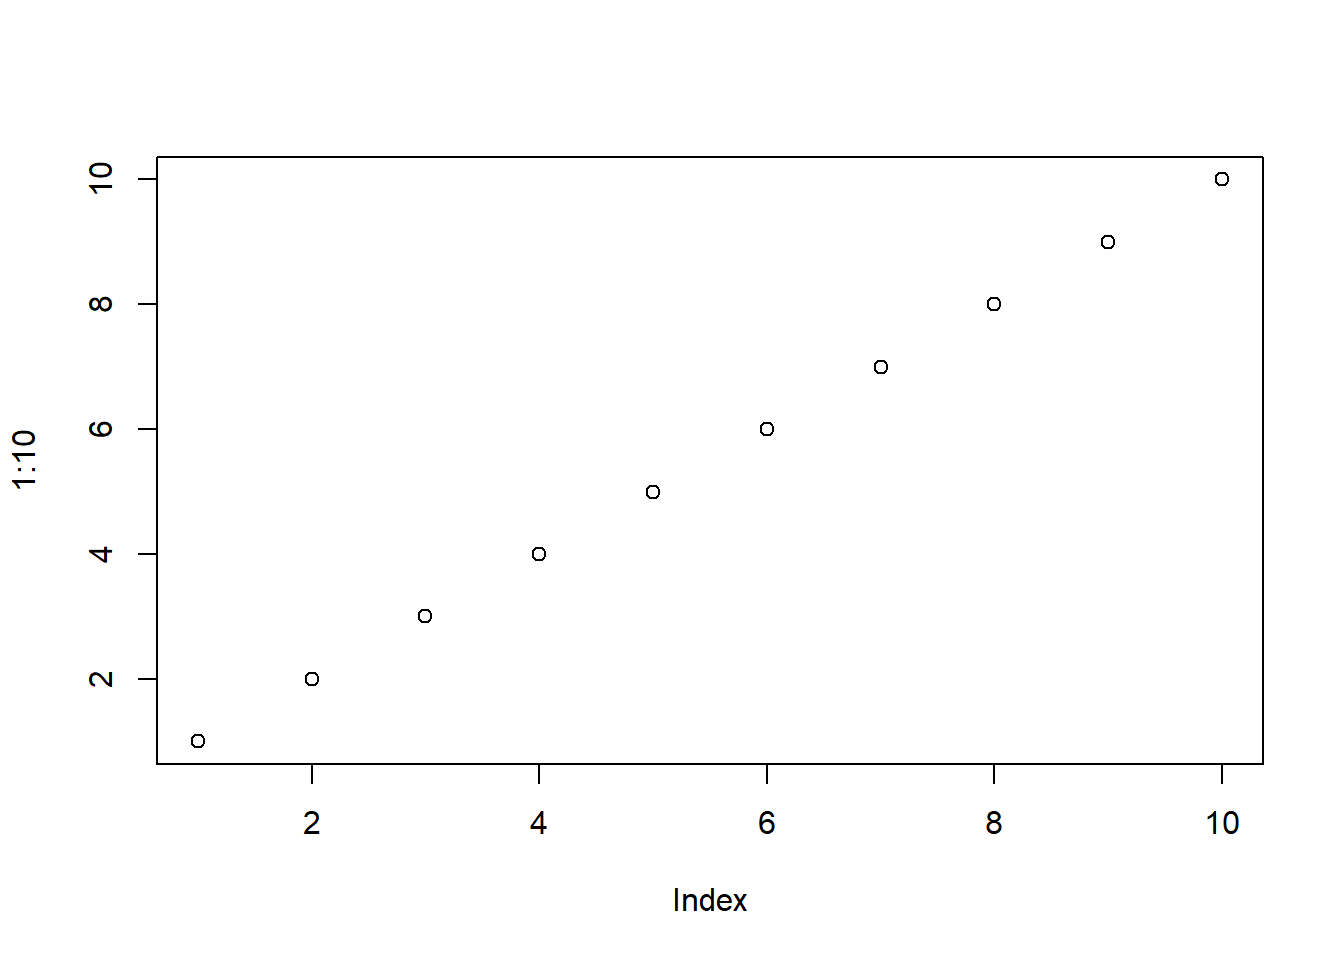
\includegraphics{Cluster-and-PCA_files/figure-pdf/unnamed-chunk-1-1.pdf}

}

\end{figure}

Let's get 30 points with a mean of 3 and another 30 points with a mean
of -3. Combine two results into a vector.

\begin{Shaded}
\begin{Highlighting}[]
\NormalTok{distrib }\OtherTok{\textless{}{-}} \FunctionTok{c}\NormalTok{(}\FunctionTok{rnorm}\NormalTok{(}\DecValTok{30}\NormalTok{, }\AttributeTok{mean=}\DecValTok{3}\NormalTok{),}\FunctionTok{rnorm}\NormalTok{(}\DecValTok{30}\NormalTok{, }\AttributeTok{mean=}\SpecialCharTok{{-}}\DecValTok{3}\NormalTok{))}
\end{Highlighting}
\end{Shaded}

Combine the vector and its reverse version into a matrix

\begin{Shaded}
\begin{Highlighting}[]
\NormalTok{x }\OtherTok{\textless{}{-}} \FunctionTok{cbind}\NormalTok{(distrib,}\FunctionTok{rev}\NormalTok{(distrib))}
\FunctionTok{plot}\NormalTok{(x)}
\end{Highlighting}
\end{Shaded}

\begin{figure}[H]

{\centering 
\includegraphics{Cluster-and-PCA_files/figure-pdf/unnamed-chunk-3-1.pdf}

}

\end{figure}

\hypertarget{k-means-clustering}{%
\subsection{k-means clustering}\label{k-means-clustering}}

very popular clustering method that we can use with the
\texttt{kmeans()} function in base R.

\begin{Shaded}
\begin{Highlighting}[]
\NormalTok{km }\OtherTok{\textless{}{-}} \FunctionTok{kmeans}\NormalTok{(x,}\AttributeTok{centers =} \DecValTok{2}\NormalTok{)}
\NormalTok{km}
\end{Highlighting}
\end{Shaded}

\begin{verbatim}
K-means clustering with 2 clusters of sizes 30, 30

Cluster means:
    distrib          
1  2.922671 -2.807807
2 -2.807807  2.922671

Clustering vector:
 [1] 1 1 1 1 1 1 1 1 1 1 1 1 1 1 1 1 1 1 1 1 1 1 1 1 1 1 1 1 1 1 2 2 2 2 2 2 2 2
[39] 2 2 2 2 2 2 2 2 2 2 2 2 2 2 2 2 2 2 2 2 2 2

Within cluster sum of squares by cluster:
[1] 59.28864 59.28864
 (between_SS / total_SS =  89.3 %)

Available components:

[1] "cluster"      "centers"      "totss"        "withinss"     "tot.withinss"
[6] "betweenss"    "size"         "iter"         "ifault"      
\end{verbatim}

Look at the available components

\begin{Shaded}
\begin{Highlighting}[]
\NormalTok{km}\SpecialCharTok{$}\NormalTok{ifault}
\end{Highlighting}
\end{Shaded}

\begin{verbatim}
[1] 0
\end{verbatim}

\begin{quote}
Q. How many points are in each clusters?
\end{quote}

\begin{Shaded}
\begin{Highlighting}[]
\NormalTok{km}\SpecialCharTok{$}\NormalTok{size}
\end{Highlighting}
\end{Shaded}

\begin{verbatim}
[1] 30 30
\end{verbatim}

\begin{quote}
Q. What `component' of your result object details? - cluster size -
cluster assignment/membership - cluster center
\end{quote}

\begin{Shaded}
\begin{Highlighting}[]
\NormalTok{km}\SpecialCharTok{$}\NormalTok{size}
\end{Highlighting}
\end{Shaded}

\begin{verbatim}
[1] 30 30
\end{verbatim}

\begin{Shaded}
\begin{Highlighting}[]
\NormalTok{km}\SpecialCharTok{$}\NormalTok{cluster}
\end{Highlighting}
\end{Shaded}

\begin{verbatim}
 [1] 1 1 1 1 1 1 1 1 1 1 1 1 1 1 1 1 1 1 1 1 1 1 1 1 1 1 1 1 1 1 2 2 2 2 2 2 2 2
[39] 2 2 2 2 2 2 2 2 2 2 2 2 2 2 2 2 2 2 2 2 2 2
\end{verbatim}

\begin{Shaded}
\begin{Highlighting}[]
\NormalTok{km}\SpecialCharTok{$}\NormalTok{centers}
\end{Highlighting}
\end{Shaded}

\begin{verbatim}
    distrib          
1  2.922671 -2.807807
2 -2.807807  2.922671
\end{verbatim}

\begin{quote}
Q. Plot x colored by the kmeans cluster assignment and add cluster
centers as blue points
\end{quote}

\begin{Shaded}
\begin{Highlighting}[]
\FunctionTok{plot}\NormalTok{(x, }\AttributeTok{col=}\NormalTok{km}\SpecialCharTok{$}\NormalTok{cluster)}
\FunctionTok{points}\NormalTok{(km}\SpecialCharTok{$}\NormalTok{centers, }\AttributeTok{col =} \StringTok{\textquotesingle{}blue\textquotesingle{}}\NormalTok{, }\AttributeTok{pch=}\DecValTok{19}\NormalTok{)}
\end{Highlighting}
\end{Shaded}

\begin{figure}[H]

{\centering 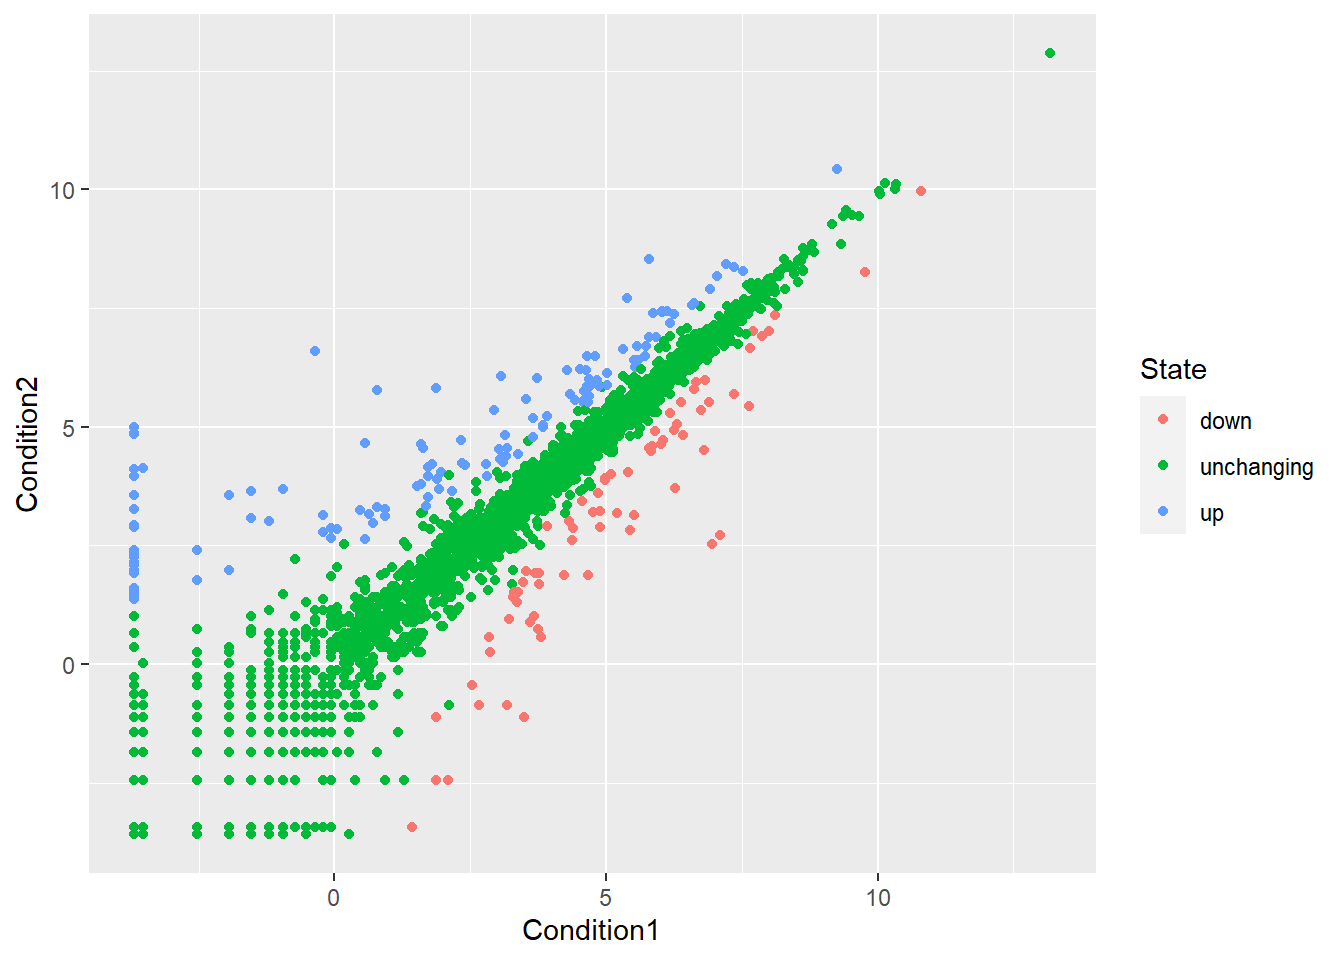
\includegraphics{Cluster-and-PCA_files/figure-pdf/unnamed-chunk-8-1.pdf}

}

\end{figure}

\begin{quote}
Q Let's cluster into 3 groups or same \texttt{x} data and make a plot
\end{quote}

\begin{Shaded}
\begin{Highlighting}[]
\NormalTok{km2 }\OtherTok{\textless{}{-}} \FunctionTok{kmeans}\NormalTok{(x, }\AttributeTok{centers=}\DecValTok{3}\NormalTok{)}
\NormalTok{km2}
\end{Highlighting}
\end{Shaded}

\begin{verbatim}
K-means clustering with 3 clusters of sizes 30, 17, 13

Cluster means:
    distrib          
1  2.922671 -2.807807
2 -2.713481  2.160243
3 -2.931158  3.919692

Clustering vector:
 [1] 1 1 1 1 1 1 1 1 1 1 1 1 1 1 1 1 1 1 1 1 1 1 1 1 1 1 1 1 1 1 3 2 2 2 2 3 3 2
[39] 2 2 3 2 3 2 2 3 2 3 2 3 3 2 3 3 3 2 2 2 2 3

Within cluster sum of squares by cluster:
[1] 59.28864 17.03278 19.10210
 (between_SS / total_SS =  91.4 %)

Available components:

[1] "cluster"      "centers"      "totss"        "withinss"     "tot.withinss"
[6] "betweenss"    "size"         "iter"         "ifault"      
\end{verbatim}

\begin{Shaded}
\begin{Highlighting}[]
\NormalTok{km2}\SpecialCharTok{$}\NormalTok{size}
\end{Highlighting}
\end{Shaded}

\begin{verbatim}
[1] 30 17 13
\end{verbatim}

\begin{Shaded}
\begin{Highlighting}[]
\FunctionTok{plot}\NormalTok{(x, }\AttributeTok{col =}\NormalTok{ km2}\SpecialCharTok{$}\NormalTok{cluster)}
\end{Highlighting}
\end{Shaded}

\begin{figure}[H]

{\centering 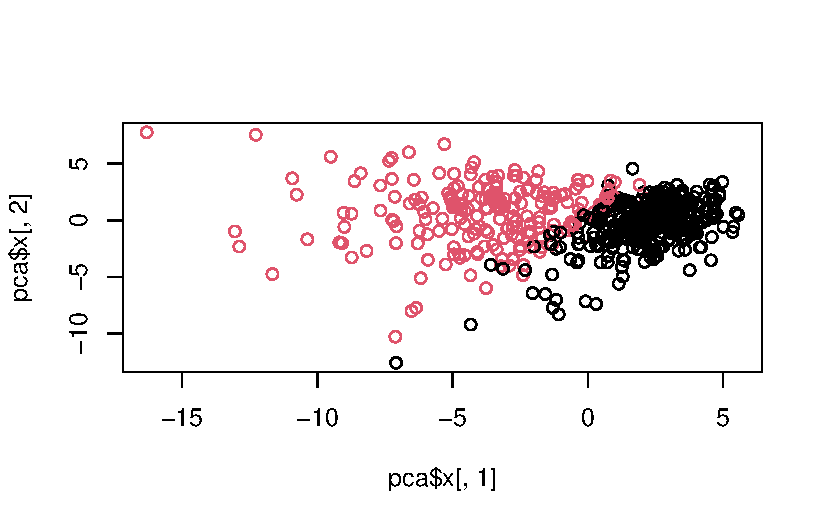
\includegraphics{Cluster-and-PCA_files/figure-pdf/unnamed-chunk-10-1.pdf}

}

\end{figure}

How do we know what number of centers(clusters) are the best

\begin{Shaded}
\begin{Highlighting}[]
\NormalTok{km2}\SpecialCharTok{$}\NormalTok{totss}
\end{Highlighting}
\end{Shaded}

\begin{verbatim}
[1] 1103.729
\end{verbatim}

\hypertarget{hierarchicalclustering}{%
\subsection{Hierarchicalclustering}\label{hierarchicalclustering}}

We can use the \texttt{hclust()} function for hierarchical clustering
unlike \texttt{kmeans()}, where we could just pass in our data as input,
weneed to give \texttt{hclust()} a ``distance matrix''.

We will use a \texttt{dist()} function to start with.

\begin{Shaded}
\begin{Highlighting}[]
\NormalTok{d }\OtherTok{\textless{}{-}}\FunctionTok{dist}\NormalTok{(x)}
\NormalTok{hc }\OtherTok{\textless{}{-}} \FunctionTok{hclust}\NormalTok{(d)}
\NormalTok{hc}
\end{Highlighting}
\end{Shaded}

\begin{verbatim}

Call:
hclust(d = d)

Cluster method   : complete 
Distance         : euclidean 
Number of objects: 60 
\end{verbatim}

Generate dendrogram

\begin{Shaded}
\begin{Highlighting}[]
\FunctionTok{plot}\NormalTok{(hc)}
\end{Highlighting}
\end{Shaded}

\begin{figure}[H]

{\centering 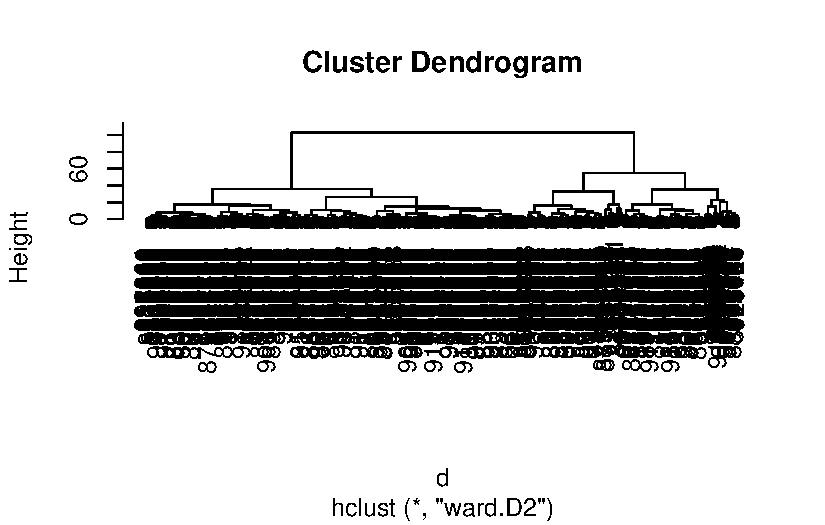
\includegraphics{Cluster-and-PCA_files/figure-pdf/unnamed-chunk-13-1.pdf}

}

\end{figure}

I can now ``cut'' my tree with the \texttt{cutree()} to yield a cluster
membership vector

\begin{Shaded}
\begin{Highlighting}[]
\NormalTok{grps }\OtherTok{\textless{}{-}} \FunctionTok{cutree}\NormalTok{(hc, }\AttributeTok{h=}\DecValTok{8}\NormalTok{)}
\NormalTok{grps}
\end{Highlighting}
\end{Shaded}

\begin{verbatim}
 [1] 1 1 1 1 1 1 1 1 1 1 1 1 1 1 1 1 1 1 1 1 1 1 1 1 1 1 1 1 1 1 2 2 2 2 2 2 2 2
[39] 2 2 2 2 2 2 2 2 2 2 2 2 2 2 2 2 2 2 2 2 2 2
\end{verbatim}

\begin{Shaded}
\begin{Highlighting}[]
\FunctionTok{plot}\NormalTok{(x, }\AttributeTok{col=}\NormalTok{grps)}
\end{Highlighting}
\end{Shaded}

\begin{figure}[H]

{\centering 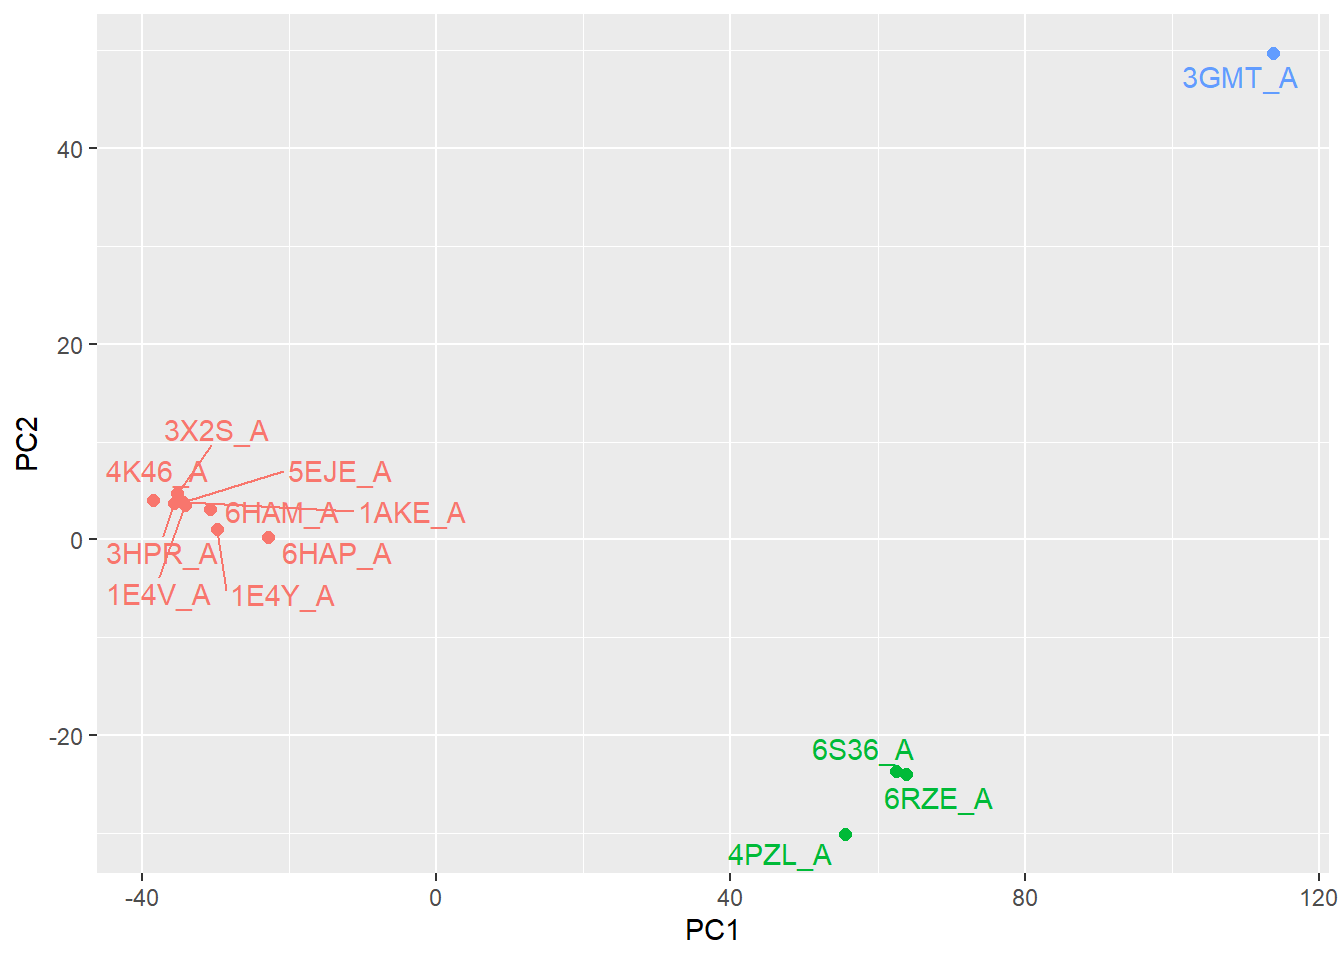
\includegraphics{Cluster-and-PCA_files/figure-pdf/unnamed-chunk-14-1.pdf}

}

\end{figure}

You can also tell \texttt{cutree()} to cut where it yields ``k'' groups

\begin{Shaded}
\begin{Highlighting}[]
\FunctionTok{cutree}\NormalTok{(hc, }\AttributeTok{k=}\DecValTok{2}\NormalTok{)}
\end{Highlighting}
\end{Shaded}

\begin{verbatim}
 [1] 1 1 1 1 1 1 1 1 1 1 1 1 1 1 1 1 1 1 1 1 1 1 1 1 1 1 1 1 1 1 2 2 2 2 2 2 2 2
[39] 2 2 2 2 2 2 2 2 2 2 2 2 2 2 2 2 2 2 2 2 2 2
\end{verbatim}

\hypertarget{principal-component-analysis-pca}{%
\section{Principal Component Analysis
(PCA)}\label{principal-component-analysis-pca}}

PCA of UK food data

\begin{Shaded}
\begin{Highlighting}[]
\NormalTok{uk }\OtherTok{\textless{}{-}} \FunctionTok{read.csv}\NormalTok{(}\StringTok{"https://tinyurl.com/UK{-}foods"}\NormalTok{, }\AttributeTok{row.names=}\DecValTok{1}\NormalTok{)}
\NormalTok{uk}
\end{Highlighting}
\end{Shaded}

\begin{verbatim}
                    England Wales Scotland N.Ireland
Cheese                  105   103      103        66
Carcass_meat            245   227      242       267
Other_meat              685   803      750       586
Fish                    147   160      122        93
Fats_and_oils           193   235      184       209
Sugars                  156   175      147       139
Fresh_potatoes          720   874      566      1033
Fresh_Veg               253   265      171       143
Other_Veg               488   570      418       355
Processed_potatoes      198   203      220       187
Processed_Veg           360   365      337       334
Fresh_fruit            1102  1137      957       674
Cereals                1472  1582     1462      1494
Beverages                57    73       53        47
Soft_drinks            1374  1256     1572      1506
Alcoholic_drinks        375   475      458       135
Confectionery            54    64       62        41
\end{verbatim}

\begin{quote}
Q1. How many rows and columns are in your new data frame named x? What R
functions could you use to answer this questions?
\end{quote}

\begin{Shaded}
\begin{Highlighting}[]
\FunctionTok{dim}\NormalTok{(uk)}
\end{Highlighting}
\end{Shaded}

\begin{verbatim}
[1] 17  4
\end{verbatim}

\begin{Shaded}
\begin{Highlighting}[]
\FunctionTok{ncol}\NormalTok{(uk)}
\end{Highlighting}
\end{Shaded}

\begin{verbatim}
[1] 4
\end{verbatim}

\begin{Shaded}
\begin{Highlighting}[]
\FunctionTok{nrow}\NormalTok{(uk)}
\end{Highlighting}
\end{Shaded}

\begin{verbatim}
[1] 17
\end{verbatim}

Preview the first 6 rows

\begin{Shaded}
\begin{Highlighting}[]
\FunctionTok{head}\NormalTok{(uk)}
\end{Highlighting}
\end{Shaded}

\begin{verbatim}
               England Wales Scotland N.Ireland
Cheese             105   103      103        66
Carcass_meat       245   227      242       267
Other_meat         685   803      750       586
Fish               147   160      122        93
Fats_and_oils      193   235      184       209
Sugars             156   175      147       139
\end{verbatim}

\begin{quote}
Q2. Which approach to solving the `row-names problem' mentioned above do
you prefer and why? Is one approach more robust than another under
certain circumstances?
\end{quote}

Using the row.names argument of read.csv(). Using \texttt{-} to delete
rows will affect the original code and delete one row every time I run
the code.

Generating a bar-plot for the data:

\begin{Shaded}
\begin{Highlighting}[]
\FunctionTok{barplot}\NormalTok{(}\FunctionTok{as.matrix}\NormalTok{(uk), }\AttributeTok{beside=}\NormalTok{T, }\AttributeTok{col=}\FunctionTok{rainbow}\NormalTok{(}\FunctionTok{nrow}\NormalTok{(uk)))}
\end{Highlighting}
\end{Shaded}

\begin{figure}[H]

{\centering 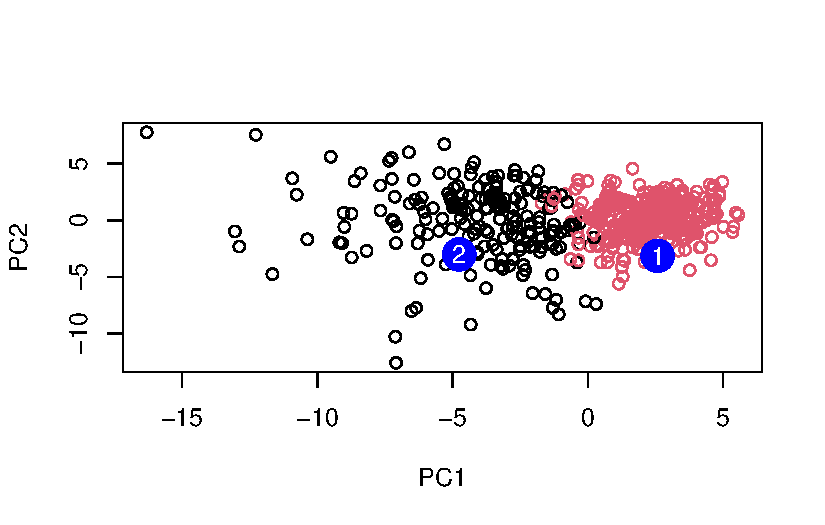
\includegraphics{Cluster-and-PCA_files/figure-pdf/unnamed-chunk-19-1.pdf}

}

\end{figure}

\begin{quote}
Q3: Changing what optional argument in the above barplot() function
results in the following plot?
\end{quote}

change beside from T to F

\begin{Shaded}
\begin{Highlighting}[]
\FunctionTok{barplot}\NormalTok{(}\FunctionTok{as.matrix}\NormalTok{(uk), }\AttributeTok{beside=}\NormalTok{F, }\AttributeTok{col=}\FunctionTok{rainbow}\NormalTok{(}\FunctionTok{nrow}\NormalTok{(uk)))}
\end{Highlighting}
\end{Shaded}

\begin{figure}[H]

{\centering \includegraphics{Cluster-and-PCA_files/figure-pdf/unnamed-chunk-20-1.pdf}

}

\end{figure}

\begin{quote}
Q5: Generating all pairwise plots may help somewhat. Can you make sense
of the following code and resulting figure? What does it mean if a given
point lies on the diagonal for a given plot.
\end{quote}

\texttt{pairs()} produce a matrix of scatterplot.

\begin{Shaded}
\begin{Highlighting}[]
\FunctionTok{pairs}\NormalTok{(uk, }\AttributeTok{col=}\FunctionTok{rainbow}\NormalTok{(}\DecValTok{17}\NormalTok{), }\AttributeTok{pch=}\DecValTok{16}\NormalTok{)}
\end{Highlighting}
\end{Shaded}

\begin{figure}[H]

{\centering \includegraphics{Cluster-and-PCA_files/figure-pdf/unnamed-chunk-21-1.pdf}

}

\end{figure}

Points lying on the diagonal means that the consumption of foods for two
countries are similar.

\hypertarget{use-pca}{%
\subsubsection{Use PCA}\label{use-pca}}

Use the \texttt{prcomp()} PCA function, it expect the transpose of our
data. \texttt{t()} returns a transpose of data.frame (col becomes row,
row becomes col).

\begin{Shaded}
\begin{Highlighting}[]
\NormalTok{pca }\OtherTok{\textless{}{-}} \FunctionTok{prcomp}\NormalTok{( }\FunctionTok{t}\NormalTok{(uk) )}
\FunctionTok{summary}\NormalTok{(pca)}
\end{Highlighting}
\end{Shaded}

\begin{verbatim}
Importance of components:
                            PC1      PC2      PC3       PC4
Standard deviation     324.1502 212.7478 73.87622 4.189e-14
Proportion of Variance   0.6744   0.2905  0.03503 0.000e+00
Cumulative Proportion    0.6744   0.9650  1.00000 1.000e+00
\end{verbatim}

Proportion of variance means how much dimentional variance is captured
by the axis PC1.

Collectively PC1 and PC2 together capture 96\% of the original 17
dimensional variance. Thus these first two new principal axis (PC1 and
PC2) represent useful ways to view and further investigate our data set.

\begin{Shaded}
\begin{Highlighting}[]
\FunctionTok{attributes}\NormalTok{(pca)}
\end{Highlighting}
\end{Shaded}

\begin{verbatim}
$names
[1] "sdev"     "rotation" "center"   "scale"    "x"       

$class
[1] "prcomp"
\end{verbatim}

\begin{quote}
Q7. Complete the code below to generate a plot of PC1 vs PC2. The second
line adds text labels over the data points.
\end{quote}

\begin{Shaded}
\begin{Highlighting}[]
\NormalTok{pca}\SpecialCharTok{$}\NormalTok{x[,}\DecValTok{1}\NormalTok{] }\CommentTok{\# stands for the position of each country on PC1}
\end{Highlighting}
\end{Shaded}

\begin{verbatim}
   England      Wales   Scotland  N.Ireland 
-144.99315 -240.52915  -91.86934  477.39164 
\end{verbatim}

\begin{Shaded}
\begin{Highlighting}[]
\NormalTok{pca}\SpecialCharTok{$}\NormalTok{x[,}\DecValTok{2}\NormalTok{] }\CommentTok{\# stands for the position of each country on PC2}
\end{Highlighting}
\end{Shaded}

\begin{verbatim}
    England       Wales    Scotland   N.Ireland 
   2.532999  224.646925 -286.081786   58.901862 
\end{verbatim}

\begin{Shaded}
\begin{Highlighting}[]
\FunctionTok{plot}\NormalTok{(pca}\SpecialCharTok{$}\NormalTok{x[,}\DecValTok{1}\NormalTok{],pca}\SpecialCharTok{$}\NormalTok{x[,}\DecValTok{2}\NormalTok{], }\AttributeTok{col=}\FunctionTok{c}\NormalTok{(}\StringTok{"red"}\NormalTok{, }\StringTok{"orange"}\NormalTok{, }\StringTok{"green"}\NormalTok{, }\StringTok{"blue"}\NormalTok{), }
     \AttributeTok{pch=}\DecValTok{1}\NormalTok{,}
     \AttributeTok{xlab =} \StringTok{"PC1"}\NormalTok{, }\AttributeTok{ylab =} \StringTok{"PC2"}\NormalTok{)}
\FunctionTok{text}\NormalTok{(pca}\SpecialCharTok{$}\NormalTok{x[,}\DecValTok{1}\NormalTok{], pca}\SpecialCharTok{$}\NormalTok{x[,}\DecValTok{2}\NormalTok{], }\FunctionTok{colnames}\NormalTok{(uk),}
     \AttributeTok{col=}\FunctionTok{c}\NormalTok{(}\StringTok{"red"}\NormalTok{, }\StringTok{"orange"}\NormalTok{, }\StringTok{"green"}\NormalTok{, }\StringTok{"blue"}\NormalTok{))}
\end{Highlighting}
\end{Shaded}

\begin{figure}[H]

{\centering \includegraphics{Cluster-and-PCA_files/figure-pdf/unnamed-chunk-25-1.pdf}

}

\end{figure}



\end{document}
